    \documentclass[krantz1,ChapterTOCs]{krantz}
\usepackage{fixltx2e,fix-cm}
\usepackage{amssymb}
\usepackage{amsmath}
\usepackage{graphicx}
\usepackage{subfigure}
\usepackage{makeidx}
\usepackage{multicol}
\usepackage{hyperref}
\usepackage{xcolor}

\begin{document}

\begin{enumerate}    
    \item Please compute for all values of $q$ the quantities $\mathbb{E}(R|q)$ and $\mathbb{V}(R|q)$
    \begin{table}[ht!]
        \centering
        \begin{tabular}{c|ccc}
             & q= -1 & q=0 & q=1  \\
             \hline
        r=-2 & 0.10  & 0.90 & 0.25 \\
        r=-1 & 0.57  & 0.05 & 0.25 \\
        r= 0 & 0.13  & 0.05 & 0.25 \\
        r= 1 & 0.20  & 0.00 & 0.25 \\
        \end{tabular}
    \end{table}
    \begin{enumerate}
        \item {\color{red}
        \begin{align}
            &\begin{aligned}
                &\mathbb{E}(R|q=-1) = -2 p(R=-2 | q=-1) + -1 p(R=-1 | q=-1)\\
                &+ 0 p(R=0 | q=-1) + 1 p(R=1 | q=-1) \\
            \end{aligned}\\
            & = -2 (0.1) + -1 (0.57) + 0 (0.13) + 1 (0.20)\\
            & = -0.57\\
            \end{align}
            \begin{align}
            &\begin{aligned}
                &\mathbb{E}(R|q=0) = -2 p(R=-2 | q=0) + -1 p(R=-1 | q=0)\\
                &+ 0 p(R=0 | q=0) + 1 p(R=1 | q=0) \\
            \end{aligned}\\
            & = -2 (0.90) + -1 (0.05) + 0 (0.05) + 1 (0.00)\\
            & = -1.85\\
        \end{align} 
        \begin{align}
            &\begin{aligned}
                &\mathbb{E}(R|q=0) = -2 p(R=-2 | q=1) + -1 p(R=-1 | q=1)\\
                &+ 0 p(R=0 | q=1) + 1 p(R=1 | q=1) \\
            \end{aligned}\\
            & = -2 (0.25) + -1 (0.25) + 0 (0.25) + 1 (0.25)\\
            & = -0.50\\
        \end{align} 
        
        
        \begin{align*}
            &\begin{aligned}
                &\mathbb{V}(R|q=-1) = (-2+0.57)^2 p(R=-2 | q=-1) + (-1+0.57)^2 p(R=-1 | q=-1)\\
                &+ (0+0.57)^2 p(R=0 | q=-1) + (1+0.57)^2 p(R=1 | q=-1) \\
            \end{aligned}\\
            & = (-2+0.57)^2 (0.1) + (-1+0.57)^2 (0.57) + (0+0.57)^2 (0.13) + (1+0.57)^2 (0.20)\\
            & = 0.845\\
            \end{align*}
            \begin{align*}
            &\begin{aligned}
                &\mathbb{V}(R|q=0) = (-2+1.85)^2 p(R=-2 | q=0) + (-1+1.85)^2 p(R=-1 | q=0)\\
                &+ (0+1.85)^2 p(R=0 | q=0) + (1+1.85)^2 p(R=1 | q=0) \\
            \end{aligned}\\
            & = (-2+1.85)^2 (0.90) + (-1+1.85)^2 (0.05) + (0+1.85)^2 (0.05) + (1+1.85)^2 (0.00)\\
            & = 0.227\\
        \end{align*} 
        \begin{align*}
            &\begin{aligned}
                &\mathbb{V}(R|q=0) = (-2+0.50)^2 p(R=-2 | q=1) + (-1+0.50)^2 p(R=-1 | q=1)\\
                &+ (0+0.50)^2 p(R=0 | q=1) + (1+0.50)^2 p(R=1 | q=1) \\
            \end{aligned}\\
            & = (-2+0.50)^2 (0.25) + (-1+0.50)^2 (0.25) + (0+0.50)^2 (0.25) + (1+0.50)^2 (0.25)\\
            & = 1.25\\
        \end{align*} 
        
        
        }
    \end{enumerate}
    
    
    \item For the above table, why do the columns sum to the value one but the rows do not?
    
    \begin{enumerate}
        \item {\color{red}
        The columns sum to one because we are restricting the sample space to outcomes that include when the random variable Q equals the value negative one and values within a column compute the probability of R for all values in the support of R. The probability that R takes some value must sum to one.\\
        
        Values across a row are probabilities of a single value of R for different conditions on Q. No guarantee can be made here except that the values must be between zero and one.\\
        
        (i would be EXTREMELY generous here)
        }
    \end{enumerate}
    
    \item Suppose we collected the following dataset
    \begin{table}[ht!]
        \centering
        \begin{tabular}{c|c}
            x & y \\
            \hline
            -2  & -2.83  \\ 
            0   &  -0.78 \\ 
            2   &  2.83  \\ 
            1   &  0.74  \\ 
            0   &  0.67  \\ 
            1   &  2.48  \\ 
            2   &  2.52  \\ 
            3   &  3.75  \\ 
            -1  &  -0.91 \\ 
            -2  &  -1.42 \\ 
        \end{tabular}
    \end{table}
    
        \item Please compute all fitted values
        \begin{enumerate}
            \item {\color{red}
            
            \begin{align}
                \hat{\beta_{1}} = \frac{\sum_{i=1}^{n}  (y_{i} - \bar{y}) (x_{i} - \bar{x})}{\sum_{i=1}^{n} (x_{i} - \bar{x})^{2} } = 1.2\\
                \hat{\beta_{0}} = \bar{y} - \hat{\beta_{1}}\bar{x} = 0.2
            \end{align}
            Then, fitted values are
            \begin{align}
                \hat{y_{i}} = \hat{\beta_{0}} + \beta{1} x_{i}
            \end{align}
            and so 
            \begin{table}[ht!]
        \centering
        \begin{tabular}{c|c|c}
            x & y & $\hat{y}$\\
            \hline
            -2  & -2.83  & -2.2\\ 
            0   &  -0.78 & 0.2\\ 
            2   &  2.83  & 2.6\\ 
            1   &  0.74  & 1.4\\ 
            0   &  0.67  & 0.2\\ 
            1   &  2.48  & 1.4\\ 
            2   &  2.52  & 2.6\\ 
            3   &  3.75  & 3.8\\ 
            -1  &  -0.91 & -1.0\\ 
            -2  &  -1.42 & -2.2\\ 
        \end{tabular}
    \end{table}
            }
        \end{enumerate}

        
        
        \item Please compute all residuals
        \begin{enumerate}
            \item {\color{red}
            
            The formula for residuals is 
            \begin{align}
                \epsilon_{i} = y_{i} - \hat{y_{i}}
            \end{align}
            and so
            \begin{tabular}{c|c|c|c}
            x & y & $\hat{y}$ & $\epsilon$\\
            \hline
            -2  & -2.83  & -2.2& -0.6\\ 
            0   &  -0.78 & 0.2& -1.0\\ 
            2   &  2.83  & 2.6 & 0.2\\ 
            1   &  0.74  & 1.4 & -0.7\\ 
            0   &  0.67  & 0.2& 0.5\\ 
            1   &  2.48  & 1.4 & 1.1\\ 
            2   &  2.52  & 2.6 & -0.1\\ 
            3   &  3.75  & 3.8 & -0.05\\ 
            -1  &  -0.91 & -1.0& 0.1\\ 
            -2  &  -1.42 & -2.2 & 0.8\\ 
        \end{tabular}
    \end{table}
            
            }
        \end{enumerate}

\begin{enumerate}
        \item Plot residuals vs fitted values
        \begin{enumerate}
            \item {\color{red}
            See attachment in email 
            }
        \end{enumerate}


        \item Plot residuals vs the order that the data was collected where the top row was the first collected data point and the last row in the table was the 10th data point collected. 
            \begin{enumerate}
            \item {\color{red}
            
            See attachment in email
            
            }
        \end{enumerate}


    
        \item Does the linearity assumption appear to hold for this dataset? Why or why not?
            \begin{enumerate}
            \item {\color{red}
            
            The linearity assumption does appear to hold because the residuals are scattered around zero with no clear pattern
            }
        \end{enumerate}


        \item Does the equal variances assumption appear to hold? Why or why not?
        \begin{enumerate}
            \item {\color{red}
            
            The equal variances assumption does appear to hold because the residuals are scattered with no clear pattern, and because the range of the residuals is fairly constant for different fitted values.
            }
        \end{enumerate}

    
    \item Suppose we build a scatter plot of the relationship between observations of a variable $x$ and variable $y$. 
    We decide to fit a linear regression and add to the plot $\mathbb{E}(Y|x)$. 
    
    \begin{figure}[ht!]
        \centering
        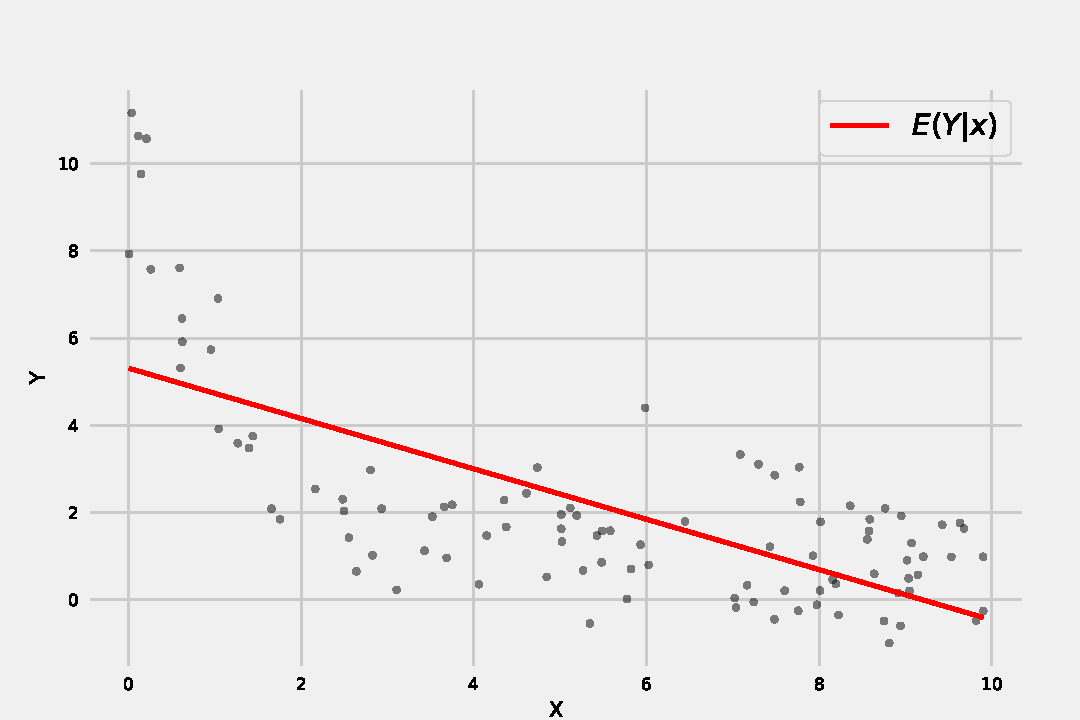
\includegraphics{chapters/chapter7/nonlinear_relationship.pdf}
    \end{figure}
    
    Please sketch what you would expect the residual vs fitted value plot to look like.
    
    \item Suppose that you fit a linear regression model and compute the residuals.
    As the residuals move closer to the line $\mathbb{E}(Y|x)$ will your estimate of $\sigma^{2}$ be smaller or larger? Why?  
    
    \item A linear regression is fit to a dataset where we collected the number of lbs of sugar an undergraduate student consumes during a week in the Fall semester and their H1Ac level.
    We estimate our parameters and find that $\hat{\beta_{0}} = 2$ and $\hat{\beta_{1}} = 10$. It may (or may not) be more reasonable to express the change in H1Ac not in increments of 1lb but instead in increments of 1 ounce.
    Please reexpress the estimated change in H1Ac in ounces of sugar consumed.  
    
    \item Will different parameter estimates lead to different diagnostic plots? Why or why not?
    
\end{enumerate} 


\end{document}